%% LaTeX2e class for student theses
%% sections/content.tex
%% 
%% Karlsruhe Institute of Technology
%% Institute for Program Structures and Data Organization
%% Chair for Software Design and Quality (SDQ)
%%
%% Dr.-Ing. Erik Burger
%% burger@kit.edu
%%
%% Version 1.3.3, 2018-04-17

\chapter{Background}
\label{ch:Background}

% TODO longer introductory paragraph?
This chapter provides background information
on several concepts that are important to the rest of the thesis.
The sections below are not intended to be comprehensive introductions to the respective topics,
but focus on the aspects that are necessary to understand the thesis.
More information can be found in the bibliography. % TODO this sentence feels weird. the bibliography doesn’t have more information, it just points you to it

\section{Wikidata}
\label{sec:Background:Wikidata}

Wikidata \cite{Vrandecic:2014:WFC:2661061.2629489} % TODO is that the best place for this \cite{}?
is a free knowledge base
and part of the Wikimedia family of sister projects,
the most famous of which is Wikipedia, the free encyclopedia.
Its contents are created, maintained and managed by the Wikidata community,
most of whose members are volunteers,
as well as the members of Wikidata’s sister projects, e.~g. Wikipedia.
Anyone can contribute to Wikidata,
but the community ensures the quality of the contents with various quality control mechanisms.
Providing another such mechanism is part of the motivation for this thesis. % TODO for this work?

Information on Wikidata is collected in items,
which represent things or concepts:
there are items for individual persons,
for cities, states, geographical features,
for organizations and corporations,
items for books, films, newspapers, journals, scientific articles,
for abstract concepts, phenomena, emotions, philosophical movements, political orientations,
items for conceptual hierarchies, parent classes, biological taxa,
and even items for fictional characters, places, or other entities.

All of these items follow the same structure.
They are identified by their item ID,
a consecutive number prefixed with the letter “Q”
(e.~g. \Q{Q188709} for Beethoven’s Symphony No. 5).
They can have a label, description, and search aliases in various languages:
for example, \Q{Q7251} is labeled “Alan Turing” in English
but «\foreignlanguage{russian}{Алан Тьюринг}» in Russian;
is described as a “British mathematician, logician, cryptanalyst, and computer scientist” in English;
and may also be found under search aliases like “Alan M. Turing”, “Alan Mathison Turing” or simply “Turing”.
They also have a set of sitelinks
(links to pages about the same concept in various other Wikimedia projects –
Wikipedia articles, Wikiquote pages, Wikimedia Commons galleries, etc.),
and most importantly, a set of statements.

The statements are where most of the information in Wikidata is stored.
They consist of a property, such as “place of birth” or “author” or “population”,
and a value, which can be a reference to another item, a quantity, a point in time, a piece of text,
or a few other possible types.
A statement can also have qualifiers
(further property-value pairs, e.~g. clarifying when or where the statement is valid)
and references (sets of property-value pairs, listing sources for the statement),
but those are mostly ignored in the context of this thesis.
Properties are also identified by an ID
(prefixed with the letter “P” instead of “Q”)
and can also have labels, descriptions and aliases in different languages:
for example, \P{P31} is labeled “instance of” in English
and „\foreignlanguage{ngerman}{ist ein(e)}“ in German.
The labels and descriptions are necessary to understand the meaning of statements,
but they are not themselves part of the statements:
statements only list references to property and item IDs,
making most of the information in Wikidata language-agnostic \cite{Kaffee:2017:GBA:3125433.3125465}.

% TODO refer to this figure somewhere in the text
\begin{figure}
  \captionsetup{singlelinecheck=off}
  \caption[Two screenshots of the same item viewed in different languages.]{
    Two screenshots of the same item viewed in different languages.
    % TODO mention the revision ID? 704641959

    The page structure is the same regardless of language.
    First, there is a heading, showing the label in the current language and the item ID.
    Below it on the left side is the “term box”,
    listing labels, descriptions and aliases in several languages relevant to the user.
    Below that is the list of statements.
    To the right are lists of sitelinks for different Wikimedia projects.

    The screenshots are truncated and do not show the full list of statements,
    but the statements pictured are:
    \begin{itemize}
    \item A statement for the property \P{P31},
      where the value is an item, \Q{Q33146843}.
    \item A statement for the property \P{P18},
      where the value is a media file on Wikimedia Commons.
      Image credit:
      \href{https://commons.wikimedia.org/wiki/User:Mariarosafg}{Mariarosafg}
      (\url{https://commons.wikimedia.org/wiki/File:Ciutat_de_Montblanc.jpg}),
      “Ciutat de Montblanc”,
      \url{https://creativecommons.org/licenses/by-sa/3.0/legalcode}
    \item Two statements for the property \P{P1448},
      where the values are monolingual text strings.
      Both statements also have qualifiers and references.
    \end{itemize}

    (The page has been lightly edited for the screenshots
    to remove some spacing and a few less relevant page elements.)
  }
  \label{fig:montblanc}
  \begin{subfigure}{\textwidth}
    \caption[The item viewed as an anonymous user in the default English language.]{
      The item viewed as an anonymous user in the default English language.
      German is shown as a second language in the term box
      because the request was made from a German IP address.
      Logged in users can configure which languages they want to be shown here.
    }
    \label{fig:montblanc-en}
    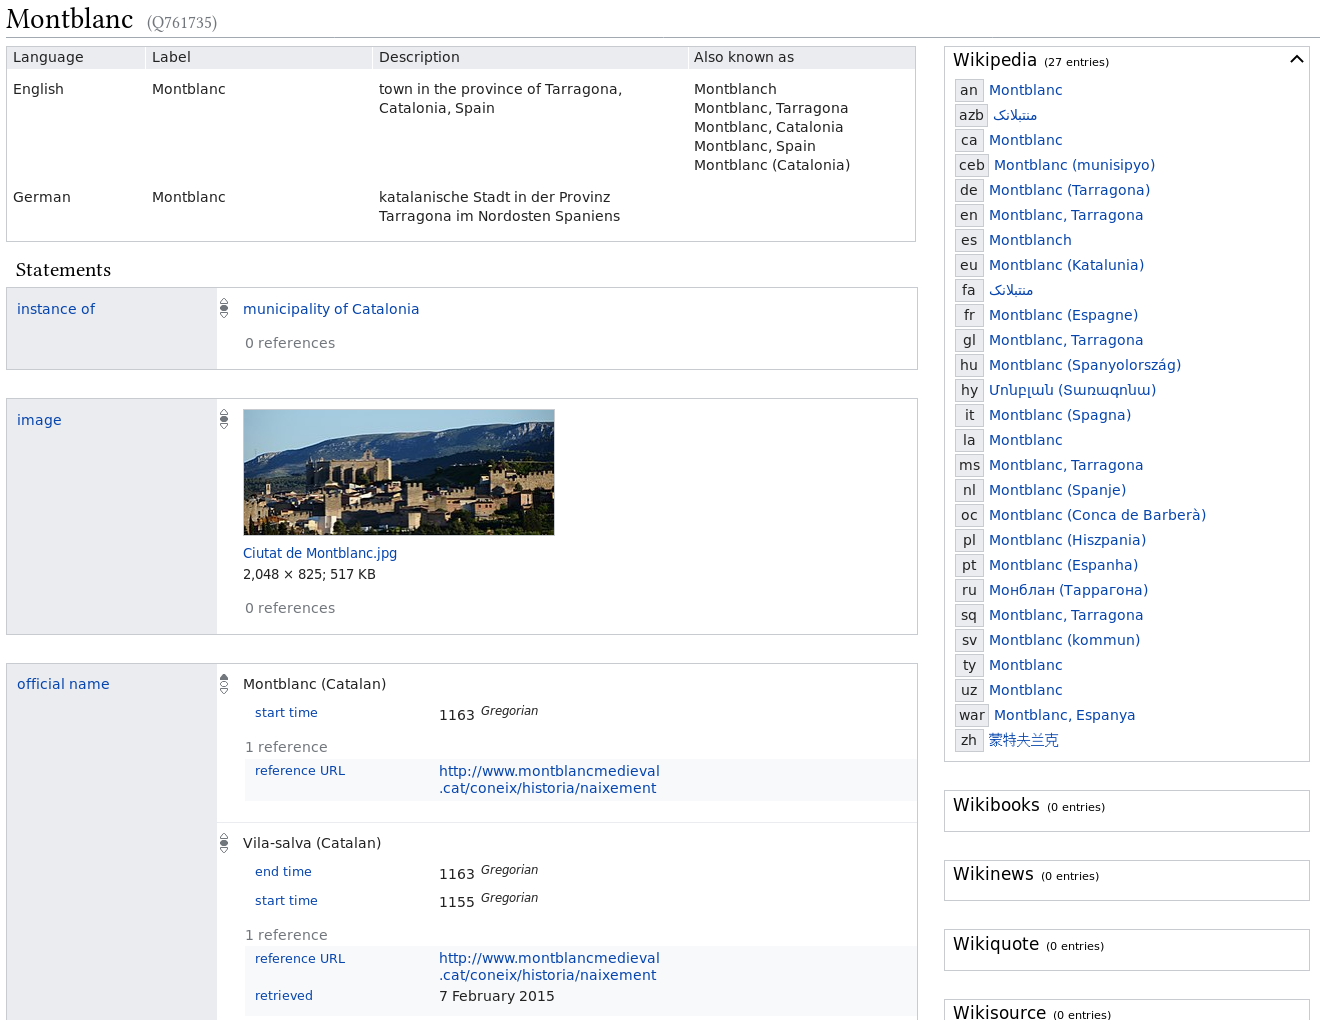
\includegraphics[width=\textwidth]{screenshots/montblanc-en}
  \end{subfigure}
\end{figure}
\begin{figure}\ContinuedFloat
  \begin{subfigure}{\textwidth}
    \caption[The item viewed as an anonymous user, explicitly requested in the Catalan language.]{
      The item viewed as an anonymous user, explicitly requested in the Catalan language.
      Notice that all property and item labels are now different.
    }
    \label{fig:montblanc-ca}
    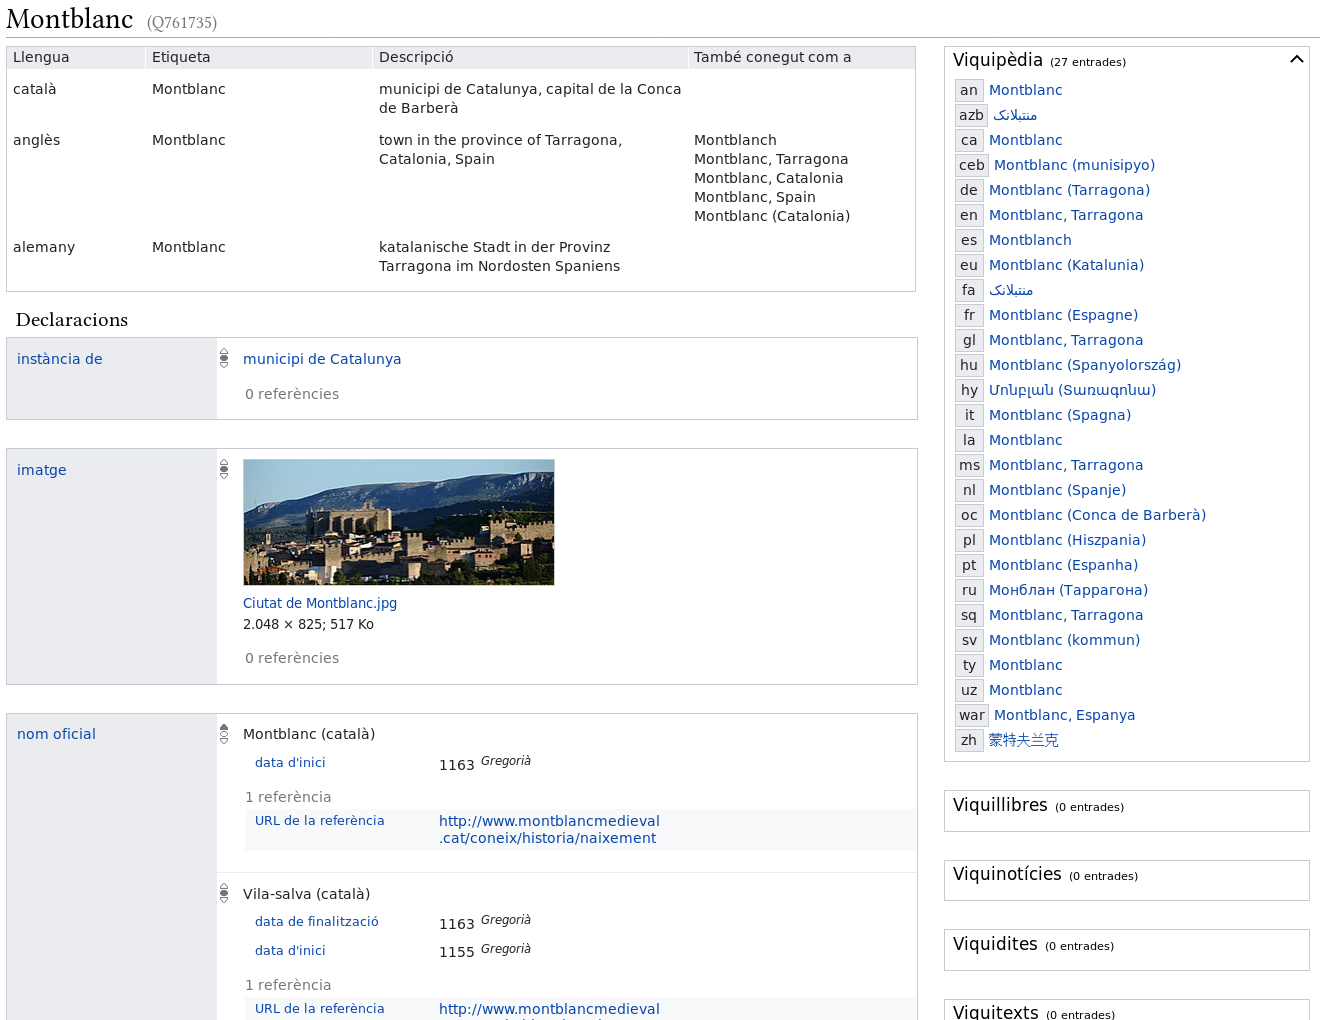
\includegraphics[width=\textwidth]{screenshots/montblanc-ca}
  \end{subfigure}
\end{figure}

It is vital to observe that there is no kind of schema inherent to the Wikidata data model.
Any property can be used on any item:
nothing in the software stops one from adding, say,
a “date of birth” statement to an item for a lake,
or a “parent taxon” statement to an item for a movie teaser poster.
The community has several ways to describe schemas to varying degrees of formality
(such as property lists on WikiProject pages or the property constraints system),
but they are all realized by community consensus,
not enforced by the Wikidata software.
The great flexibility which this lends to the community
is considered to be one of Wikidata’s greatest strengths \cite{vrandecic-restricting-the-world},
and though the use of \gls{shex}
on Wikidata will provide another,
highly formal way to describe schemas,
it is not intended to change this fundamental operating principle of Wikidata. % TODO awkward passive voice

Wikidata’s data model, as described above,
is not directly related to \gls{rdf}.
However, to enable usage of \gls{rdf} technologies and interoperation with \gls{rdf}-based datasets,
Wikidata’s data is exported to \gls{rdf}:
% TODO link to Help:Data access and query.wikidata.org? if yes, \href or \url?
the data about any item can be downloaded in various \gls{rdf} formats through a linked data interface, % TODO *the* linked data interface?
and a full, up-to-date \gls{rdf} export of Wikidata is available in the Wikidata Query Service,
a \acrshort{sparql} endpoint to which anyone may submit queries.
However, this interface is export-only:
it is not possible to edit Wikidata via \gls{rdf}.

% TODO explain some fundamental properties? P31, P279?
% TODO mention “entity” as collective term for items and properties

\section{RDF}
\label{sec:Background:RDF}

\acrfull{rdf}
\cite{Lanthaler:14:RCA}
is a framework for describing and working with linked data.
In \gls{rdf}, information is arranged in subject-predicate-object triples,
such as “<Alan Turing> <is a> <human>”
or “<Lima> <was founded in> <18 January 1535>”.
All three elements of a triple are typically URIs, % TODO acronym? URLs vs URIs vs IRIs?
but the object of a triple can also be some other kind of value,
such as a textual, numerical or other literal
(e.~g. the date literal “18 January 1535” above). % TODO blank nodes are elided for brevity, but perhaps rephrase this to make sure the text isn’t factually wrong
A collection of such triples forms a directed, labeled graph,
where the triples describe individual edges
and the nodes are the subjects and objects of the triples:
triples with the same subject constitute different outgoing arcs from the same node.
This graph can then be queried using the \acrlong{sparql} \cite{9569543}. % TODO is SPARQL really important enough to be mentioned here, and nothing else?
For a more detailed introduction,
see the RDF 1.1 Primer \cite{Schreiber:14:RP}.

% TODO should perhaps be more than one paragraph

\section{Shape Expressions}
\label{sec:Background:ShEx}

\acrfull{shex} \cite{shex}
is a standard for describing data shapes within an \gls{rdf} graph,
developed by the ShEx Community Group under the umbrella of the \gls{w3c}.
A ShEx schema consists of a number of shapes,
each of which describes a focus node,
expressing restrictions on its node kind, value, and/or incoming and outgoing links.

For example, the schema in \cref{listing:shex-example} defines two shapes,
one for humans and one for locations,
in a fictional example vocabulary.
The shape for humans describes that a human has one or more parents,
any number of children,
a date of birth,
and a place of birth;
the parents and children should also be humans,
the date of birth should be a date literal,
and the place of birth should be a location.
The shape for locations describes that a location may optionally be contained within another location.

\begin{lstfloat}
\begin{lstlisting}[language=sparql]
PREFIX ex: <http://shex.example/>

ex:Human {
  ex:parent @ex:Human+;
  ex:child @ex:Human*;
  ex:dateOfBirth xsd:dateTime;
  ex:placeOfBirth @ex:Location;
}

ex:Location {
  ex:containedWithin @ex:Location?;
}
\end{lstlisting}
\caption{A simple example schema.}
\label{listing:shex-example}
% TODO this schema is impossible to satisfy without a circular parent relationship – not a great example :/
\end{lstfloat}

% TODO this needs more content, I think
% TODO difference between v1 and v2?
% TODO ShExC? at least mention it if I use the term elsewhere

\section{RDF2Graph}
\label{sec:Background:RDF2Graph}

% TODO review the layout of the figures here

RDF2Graph % TODO glossary
\cite{vanDam2015}
is a tool to automatically determine the structure of an \gls{rdf} graph
and export it as a \gls{shex} schema
(other output formats are also supported).
It relies heavily on the type information of each node and the class hierarchy in the graph,
determining the valid predicates and their value types and cardinalities for each type in the graph.
There is also an optional step to simplify the resulting schema.

To discover the structure of an \gls{rdf} graph,
RDF2Graph runs a set of queries against a \gls{sparql} endpoint serving that graph.
(This can be a local server, perhaps simply based on a single file containing the graph,
or a remote server.)
It enumerates all the classes that occur in the graph
and then collects all the predicates that are used on instances of each class.
For each predicate of each class,
it then gets the types referenced in the values for those predicates
(usually the classes of the referenced nodes,
but values can also be literals or external references),
as well as forward and reverse multiplicity for each such type link.
All this information is stored in a separate \gls{rdf} graph private to RDF2Graph.

If the simplification step is enabled,
RDF2Graph will afterwards apply some transformations to the structure
based on the hierarchy of the classes involved,
which happens in several steps.
The following description uses the same step numbers as \cite{vanDam2015},
but elides several steps which are mostly implementation details,
which is why the step numbers are not contiguous.
See \cite{vanDam2015} and the RDF2Graph source code for the full description.
(In the source code, the steps are counted as sub-steps of the general step 7.4 “simplification”:
for example, step 2 is implemented under a code comment for “7.4.2”.)

In step 2, all predicates from child classes are copied to parent classes,
as outlined in \cref{fig:simplify-7.4.2}.

\begin{figure}[ht]
  \begin{subfigure}[t]{0.45\textwidth}
    \begin{lstlisting}
A1 extends X {
  a A;
}
A2 extends X {
  a A;
}
B extends X {
  b B;
}
X {}
    \end{lstlisting}
    \caption{Before step 2.}
    \label{fig:simplify-7.4.2-before}
  \end{subfigure}
  \begin{subfigure}[t]{0.45\textwidth}
    \begin{lstlisting}
A1 extends X {
  a A;
}
A2 extends X {
  a A;
}
B extends X {
  b B;
}
X {
  a A;
  b B;
}
    \end{lstlisting}
    \caption{After step 2.}
    \label{fig:simplify-7.4.2-after}
  \end{subfigure}
  \caption[Simplification step 2.]{Simplification step 2 (in pseudo-syntax).}
  \label{fig:simplify-7.4.2}
\end{figure}

Step 3  removes predicates which are only found in a single subclass
from the parent class again.
In the example from \cref{fig:simplify-7.4.2},
the predicate \lstinline{a} will be kept in \lstinline{X}
because it occurs in both \lstinline{A1} and \lstinline{A2},
but the predicate \lstinline{b} will be dropped
because it only occurs in the single subclass \lstinline{B} –
see \cref{fig:simplify-7.4.3}.

\begin{figure}[ht]
  \begin{subfigure}[t]{0.45\textwidth}
    \begin{lstlisting}
A1 extends X {
  a A;
}
A2 extends X {
  a A;
}
B extends X {
  b B;
}
X {
  a A;
  b B;
}
    \end{lstlisting}
    \caption{Before step 3.}
    \label{fig:simplify-7.4.3-before}
  \end{subfigure}
  \begin{subfigure}[t]{0.45\textwidth}
    \begin{lstlisting}
A1 extends X {
  a A;
}
A2 extends X {
  a A;
}
B extends X {
  b B;
}
X {
  a A;
}
    \end{lstlisting}
    \caption{After step 3.}
    \label{fig:simplify-7.4.3-after}
  \end{subfigure}
  \caption[Simplification step 3.]{Simplification step 3 (in pseudo-syntax).}
  \label{fig:simplify-7.4.3}
\end{figure}

After that, in step 4 all references which are still found in a parent class
are removed from the child classes, where they are now redundant.
See \cref{fig:simplify-7.4.4} for applying this to the same example.

\begin{figure}[ht]
  \begin{subfigure}[t]{0.45\textwidth}
    \begin{lstlisting}
A1 extends X {
  a A;
}
A2 extends X {
  a A;
}
B extends X {
  b B;
}
X {
  a A;
  b B;
}
    \end{lstlisting}
    \caption{Before step 4.}
    \label{fig:simplify-7.4.4-before}
  \end{subfigure}
  \begin{subfigure}[t]{0.45\textwidth}
    \begin{lstlisting}
A1 extends X {}
A2 extends X {}
B extends X {
  b B;
}
X {
  a A;
}
    \end{lstlisting}
    \caption{After step 4.}
    \label{fig:simplify-7.4.4-after}
  \end{subfigure}
  \caption[Simplification step 4.]{Simplification step 4 (in pseudo-syntax).}
  \label{fig:simplify-7.4.4}
\end{figure}

Step 2 also merges references to parent classes,
as outlined in \cref{fig:simplify-7.4.2-classes}.
The other steps take this into account by respecting subclass relations as well.

\begin{figure}[ht]
  \begin{subfigure}[t]{0.3\textwidth}
    \begin{lstlisting}
A1 extends A {}
A2 extends A {}
A extends B {}
    \end{lstlisting}
    \caption{The class hierarchy for this example.}
    \label{fig:simplify-7.4.2-classes-hierarchy}
  \end{subfigure}
  \begin{subfigure}[t]{0.3\textwidth}
    \begin{lstlisting}
M extends X {
  r A1
}
N extends X {
  r A2
}
O extends X {
  r B
}
X {}
    \end{lstlisting}
    \caption{Before step 2.}
    \label{fig:simplify-7.4.2-classes-before}
  \end{subfigure}
  \begin{subfigure}[t]{0.3\textwidth}
    \begin{lstlisting}
M extends X {
  r A1
}
N extends X {
  r A2
}
O extends X {
  r B
}
X {
  r B;
}
    \end{lstlisting}
    \caption{After step 2.}
    \label{fig:simplify-7.4.2-classes-after}
  \end{subfigure}
  \caption[Simplification step 2, with class relations.]{
    Simplification step 2 (in pseudo-syntax), with class relations.
    (This example is independent from the previous example.)
  }
  \label{fig:simplify-7.4.2-classes}
\end{figure}

% TODO I haven’t looked too closely into any of these steps except the very last one,
% which I practically rewrote from scratch.
% Does that show in the text? Do I need to investigate the rest of the ShEx exporter further?
At this point, the information which RDF2Graph extracted is available in a private \gls{rdf} graph.
From there, it can be exported into various formats by different exporters.
The ShEx exporter loads parts of these results into a temporary \gls{rdf} database of its own,
applies some transformations to them via \gls{sparql},
converts them to JSON-LD,
further transforms the JSON,
and finally exports the result into ShExC text via the Jade template engine.

\section{Wikimedia Toolforge}
\label{sec:Background:Toolforge}

% TODO I’m not yet sure if this section is necessary

Wikimedia Toolforge is a hosting environment provided by the Wikimedia Foundation
where trusted members of the Wikimedia community may host and develop their “tools” or other work.
Most tools are web-based and reachable under the \href{https://tools.wmflabs.org/}{tools.wmflabs.org} domain,
but it is also possible to run bots or analysis jobs on Toolforge.
Tools can be written in a variety of languages
(e.~g. PHP, Python, Java, JavaScript)
and have access to live replicas of the Wikimedia production databases,
data dumps of Wikimedia projects,
custom tool-specific databases,
and a Sun Grid Engine job execution system for long-running or resource-intensive tasks.

% TODO more text?
% TODO also mention Cloud VPS? in which case I guess the section heading would be Wikimedia Cloud Services
